\documentclass[titlepage, 13px, a4paper]{article}

\usepackage[utf8]{inputenc}

\usepackage[T1]{fontenc}
\usepackage{fontawesome}
\usepackage{eurosym}

\usepackage[french]{babel}

\usepackage{fancyhdr}
\usepackage{graphicx}
\usepackage[left=4cm,right=4cm,top=4cm,bottom=5cm,textheight=25cm]{geometry}
\usepackage{wrapfig}

\usepackage{eso-pic}
\usepackage{transparent}

\usepackage{hyperref}
\usepackage{setspace}

\usepackage{titletoc}

%\usepackage{titlesec}
%\titleformat{\part}[display]
  %{\normalfont\bfseries}{}{0pt}{\Large\bfseries}

\newcommand\BackgroundPic{%
	\put(0,-50){%
		\parbox[b][\paperheight]{\paperwidth}{%
			%\vfill
			\centering
			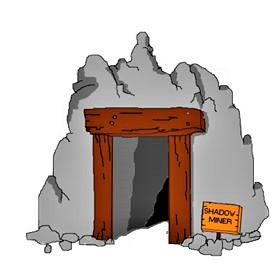
\includegraphics[%
			keepaspectratio]{../images/icone.jpg}%
			\vfill
		}
	}
}

  
\renewcommand{\baselinestretch}{1.15}
\renewcommand{\partname}{}

\title{\textbf{{\Huge Rapport de soutenance \no 1}}}
\author{
	\\
	\bsc{{\LARGE ACCEr}} \\ \\ \\
	\bsc{CLAUDEL Antoine} \\
	\bsc{FARINAZZO Cédric} \\
	\bsc{LANGUERRE Clément} \\
	\bsc{GRIZZI Edgar} \\ \\ \\
}
\date{{\LARGE \today}}

\pagestyle{fancy}
\fancyfoot[L]{
\includegraphics{../images/ShadowMiners_logo_mini.png}} %50x33
\fancyhead[R]{ACCEr}
\fancyhead[L]{Rapport de soutenance \no 1}

\begin{document}
\AddToShipoutPicture*{\BackgroundPic}

\maketitle
\tableofcontents

\newpage 

\section{Introduction} 
\paragraph{} \hspace{0pt} 
Comme chaque année à Epita, les groupes doivent créer un rapport de soutenance pour chaque soutenance. \\
Dès la validation de notre cahier des charges nous avons imaginé nos mineurs prendre vie ainsi que le naissance du vil "Shadow Miner", monstre de notre jeu et ennemi de nos ou notre mineur(s).
Ce projet a pour but de réaliser un jeu vidéo. \\
Notre projet est divisé en trois soutenances distinctes. Nous réalisons notre projet avec Unity 3D et en c\#.
Nous allons vous présenter le rapport de notre première soutenance de ce projet décrivant notre premier pas dans le monde de la programmation et de jeu vidéo 
ainsi nous retracerons l'avancée de notre projet depuis la validation de notre cahier des charges qui a eu lieu il y a environ un mois et demi. 
Notre projet est constitué d'Edgar Grizzi, Clément Languerre, Cédric farinazzo et Antoine Claudel.
Pour vous rappeler un petit peu, notre jeu est un jeu aventure survie à l'intérieur d'une mine ou notre héros un mineur doit s'échapper d'une mine 
alors qu'il est poursuivi par un monstre, Le shadow miner.
Notre jeu est constitué d'un mode solo composé d'une série de niveau et d'un mode multijoueurs où 3 joueurs s'affrontent : 
1 Shadow Miner et 2 mineurs dont un ayant la possibilité de devenir un esprit de la mine pour prendre son contrôle.


\section{Contexte} 
\paragraph{} \hspace{0pt} 
Ce projet est réalisé dans le cadre de la mise en oeuvre des connaissances acquises 
lors des cours de TD et TP informatiques et nous permet de renforcer et d’approfondir nos apprentissages.   
Actuellement, notre groupe est sur le point de passer la première soutenance.

\newpage

\part{Avancement générale}  
\section{Les objectifs remplis} 
\paragraph{} \hspace{0pt} 
Le groupe a déjà en partie bien avancé :
{\begin{enumerate}
	\item La création des préfabs est finalisé comme il était prévu dans notre planning. \\
		La création des préfabs de map pour nos niveaux comme des murs,
		des portes, des sols, des pièges et des meubles et d'autres choses pensées pour notre projet est terminée aux trois quarts.
		\\
	\item Les scripts c\# sont à jour, les personnes responsables ont fait le travail attendu pour la période d'avant première soutenance.
		Nos pics s'active au passage d'un joueur, les portes s'ouvrent lorsque nous sommes à proximité et que nous appuyons sur la touche E, ...
		\\
	\item L'objectif pour la création des niveaux était de entre 10 et 20 \%, pour l'instant cette objectif est bel et bien rempli.
			Pour la création du Shadow Miner, elle est finalisée, pour son script c\# il n'est pas commencé.
		\\
	\item Enfin la création des joueurs a aussi bien avancé.
		Nous avons récupéré un modèle 3D d'un mineur et d'un homme avec une hache pour représenté le Shadow Miner.
		Notre objectif  est donc atteint. 
		\\
	\item nous avons modélisé sous Blender quelques objets tels que des cailloux ou des pics 
		\\
	\item Pour les script c\# pour les joueurs, nous avons crée le script permettant de se déplacer avec les touches ZQSD, espace pour sauter et shift gauche + Z pour courir.
		Le joueur peut bouger la caméra en bougeant sa souris. Le joueur peut donc se déplacer librement dans les niveaux.
		Le joueur possède une script lui permettant d'avoir une vie, de prendre des dégats et d'attaquer un Game Object.
		Mais vous n'avons pas encore mis en place ce système.
		Nous avions prévu de faire 50 \% de la tache et il a été fait plus que notre objectif de départ.
		\\ \newpage	
	\item La création de notre site internet est bien entamée : nous pouvons nous connecter et ajouter des rapports. \\
		L'hébergement du site est finie et le site est accessible à l'addresse \url{https://accer.ddns.net/} .  \\
		Un version web du jeu est accessible à l'addresse \url{https:/accer.ddns.net/game/} .
		Notre but de départ était de 40 \%, avec joie nous pouvons affiremr qu'il est actuellement de 60 \%.*
		\\
	\item La création du serveur multijoueur est finalisé, le network fonctionne mais il y a quelques problèmes de synchronisation dû au temps de latence avec le serveur.
		Pour le moment, les animations ne sont synchronisé pas néanmoins l'avancée du groupe est de 40 ou 45\%.
		\\
\end{enumerate}}

\section{Objectifs futurs jusque la seconde soutenance} 
\paragraph{} \hspace{0pt} 
Nous prévoyons de finaliser tous les prefabs de map pour nos niveaux en ajoutant encore des objets tels que des rails et un ascenseur.\\
Nous continuerons la modélisation 3D pour obtenir un meilleur rendu visuel dans l'objectif de faire les trois quarts attendu. \\
Nous continuerons les scripts C\# pour les animations pour que les pièges puissent infligées des dégats au joueurs. \\
Nous améliorerons les scripts c\# des joueurs afin de créer des dégats de chute ou que le joueur puisse attaqué avec différentes armes et puisse mourir lorsque sa vie tombe à zéero.\\
Nous continuerons de créer des niveaux de plus en plus difficiles. \\
Nous entamerons les scripts c\# de l'IA du Shadow Miner afin qu'il puisse marcher, courir, nous suivre et nous attaquer.\\
Nous commencerons à créer des cinématiques comme prévu. \\
Nous ajouterons du son dans notre jeu afin que notre jeu soit plus réaliste (bruit de pas, grognements, explosions, ...). \\
Le menu du jeu sera recréé car l'actuel est temporaire.
Le site internet va s'aggrandir et nous créerons la possibilité de lier son compte au jeu afin que la progression des joueurs soit visible 
sur le site ou que le joueur puisse paramétrer son compte multijoueur depuis le site internet. \\
Enfin nous commencerons la création du système de map aléatoire pour le mode multijoueurs.

Ainsi nous remplierons nos objectifs définis dans notre cahier des charges.


\newpage

\part{Modification de l'histoire et du gameplay}

\paragraph{} \hspace{0pt}
Nous avons effectué quelques modifications sur le gameplay du jeu afin que notre jeu soit cohérent.

\section{Cinématique du mode solo}
\paragraph{} \hspace{0pt} \\
Dans le cahier des charges, nous avons proposé 2 scénarios possibles pour le mode solo. \\
Nous avons finalement choisi le 2ème scénario : 
\\
\begin{quotation}
	Un mineur descend tôt le matin dans les derniers sous-sols de la mine, là où l’oxygène se fait rare. 
	Un mineur fou (le Shadow Miner) coupe les câbles de l’ascenseur. 
	Le mineur veut alors rejoindre la surface. Le Shadow Miner va alors vouloir l’en empêcher.
	L’utilisateur incarne alors le mineur. \\
\end{quotation}

Au niveau des détail dans la mine, il y aura des salles abandonnées et des salles semblant être encore utilisées.
Le tout sera reliée par de sombres couloirs ...

\section{Précision générale}
\paragraph{} \hspace{0pt} \\
Nous avons jugé utile de précisé les touches utilsés pour joueur au jeu pour le moment (clavier azerty): 
{\begin{enumerate}
	\item Z : Avancer vers l'avant
	\item Q : Avancer vers la gauche
	\item S : Reculer
	\item D : Avancer vers la droite
	\item Shift left + Z : Courir
	\item Espace : Sauter
	\item E : Ouvrir des portes.
\end{enumerate}}

\section{Précision à propos du mode multijoueurs}
\paragraph{} \hspace{0pt} \\
Nous avons souhaité ajouté quelques précisions sur le mode multijoueurs :
\\
{\begin{enumerate}
	\item Nous utilisons Photon Unity Networking pour le multijoueurs.
		\\
	\item Le joueur devra créer un compte pour pouvoir accéder au mode multijoueurs.
			Ce compte pourra être créer sur le site internet ou dans le jeu lui-même
			Ainsi le joueur pourra consulter et modifier ses données depuis le site internet ou le jeu.
			Ce système lui permet de jouer sur une version éxécutable du jeu comme sur la version web du jeu en conservant ses données.
			Ainsi la portabilité et l'accessibilité du jeu en seront augmentée.
		\\
	\item Etant donné le nombre de joueur pouvant être connecté au serveur (20 joueurs max), donc nous prévoyons 6 rooms de jeu avec des maps aléatoires.
		\\
\end{enumerate}}


\part{Apports collectifs et personnels}
\paragraph{} \hspace{0pt} \\
Depuis le cahier des charges, cette longue période de travail nous as permis d'apprendre à utiliser Unity, 
de comprendre l'utilité du C\# dans le développement d'applications, de nous initier à la modélisation 3D et à collaborer en utilisant git.
\\
Cette partie nous apprend beaucoup de choses que nous devrons utiliser dans la suite du projet 

\newpage

\newpage
\part{Problèmes rencontrées et sources }
\section{Problèmes rencontrées}
\paragraph{} \hspace{0pt} \\
Nous n'avons pas rencontré de problème majeurs mis à part que le network n'est pas fluide (nous trouverons une solution bientôt) 
et que lors d'un changement de scène la directionnel light ne s'active pas, du coup nous avons créé une seconde directionnel light pour patcher ce bug et ca marche !


\section{Source}
\paragraph{} \hspace{0pt} \\
N'etant pas des experts en modélisation 3D, nous avons du trouvé nos personnages sur internet : 
{\begin{itemize}
	\item Le mineur provient des standarts assets de Unity 4.x, nous avons juste récupéré le modele 3D et les animations. 
	car nous n'avons pas le droit de récupérer de script et que les scripts de l'assets étaient en Javascript(Unityscript).
	\item Nous avons récupéré le Shadow Miner sur le site \url{https://www.mixamo.com/} ainsi que les animations qu'ils possède.
	Le site indique clairement que nous pouvons utiliser ces assets pour le création de jeu vidéo (\url{https://forums.adobe.com/thread/1992542}).
	\item les textures sur les objet et les sols proviennent de l'Assets Store.
\end{itemize}}

\newpage

\part{Avancement Personnel}  
\section{Antoine}
\paragraph{} \hspace{0pt} \\
\begin{wrapfigure}[7]{r}{5cm}
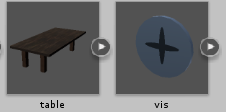
\includegraphics[width=5cm]{table-antoine.png}
\end{wrapfigure}
Antoine a réalisé son premier jeu vidéo en troisième dans le cadre du projet d'ISN. 
Il s'agissait d'un Snake, codé par groupe de trois en Python. 
\\
Aujourd'hui il s'attaque  à un jeu d'horreur. 
Avec l'équipe ACCEr, Antoine a commencé à réfléchir concrètement à ce qu'allait contenir le jeu. 
Après la remise du cahier des charges, seul le concept de « jeux d'horreur dans une mine » était fixé. 

\paragraph{} \hspace{0pt} \\
\begin{wrapfigure}[8]{l}{5cm}
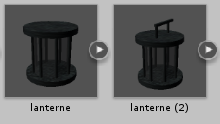
\includegraphics[width=5cm]{lanterne-ant.png}
\end{wrapfigure}
Il a donc commencé à créer quelques préfabrication (préfabs à partir de maintenant) qui serviront de base 
pour chaque niveau. Il a construit un mur en pierre composé de plusieurs cubes, avec des poutres en bois. 
Il a ensuite construit une table en bois. Les matériaux ont été trouvés sur l'asset store, 
mais tous les objets ont été fait main. Enfin il a créé une flamme avec des particules 
en suivant un tutoriel sur Youtube. Après la suspension du projet engendrée par la semaine de midterm, 
on a tous repris le travail. Antoine est en charge de la création des niveaux. \\
Il a donc élaboré un plan d'architecte pour le premier niveau, tandis qu'Edgar s'occupait du plan du second niveau. 
Les exigences du groupe étaient de commencer le niveau en sortant d'un ascenseur, qui a chuté jusqu'au dernier étage 
lors de l'introduction. Le joueur doit ensuite remonter petit à petit pour s'enfuir de la mine. 
Antoine a donc imaginé un niveau où le joueur sort d'un ascenseur, avance le long d'un couloir mal éclairé 
et découvre que le passage vers l'escalier de secours et condamné. \\
Il continue donc dans la mine en passant par un bureau où il pourra récupérer l'équipement de départ, 
c'est-à-dire une pioche et une lanterne. Il y aura des toilettes d'un côté et le chemin vers la mine de l'autre. 
Une fois arrivé dans la zone de minage le joueur descend jusqu'au fond de la mine et 
découvre un tunnel qui le conduit au niveau suivant. \\
La première déception d'Antoine apparu lorsqu'il comprit qu'il n'aurait pas le temps de finir le niveau 
avant la première soutenance. Il commença à créé une torche à partir de la flamme qu'il avait ajouté précédemment, 
puis une lanterne avec une poignée. Pour créer ces objets il est passé par des préfabs intermédiaires, 
comme des vis, des barreaux et des vitres (faites par lui-même à l'aide de tutoriels) pour la lanterne. 
Ensuite il modifia le terrain pour donner l'impression d'une zone de minage, puis il ajouta les murs et 
finalisa le squelette du premier niveau. Il le compléta en rajoutant quelques préfabs de cagette, étagères, 
table et armoire (faits par Clément). Antoine conçu également un menu temporaire du jeu avec 3 boutons : 
un vers le niveau 1, un vers le niveau 2 et un vers la scène multijoueur. \\
Malgré quelques difficultés lors du test des boutons (il manquait un public devant les fonctions C\#) 
le menu est opérationnel et Cédric a même complété le code avec l'ajout de variable modifiable depuis UNITY.

\paragraph{} \hspace{0pt} \\
Antoine prévoit de continuer à construire les autres niveaux (au minimum 5 d'ici la prochaine soutenance), 
de poursuivre le scénario et de créer les préfabs nécessaires avec l'aide des autres membres, notamment des WC 
et des minerais.

torche-ant.png
\begin{center}
	\begin{figure}[!hp]
	   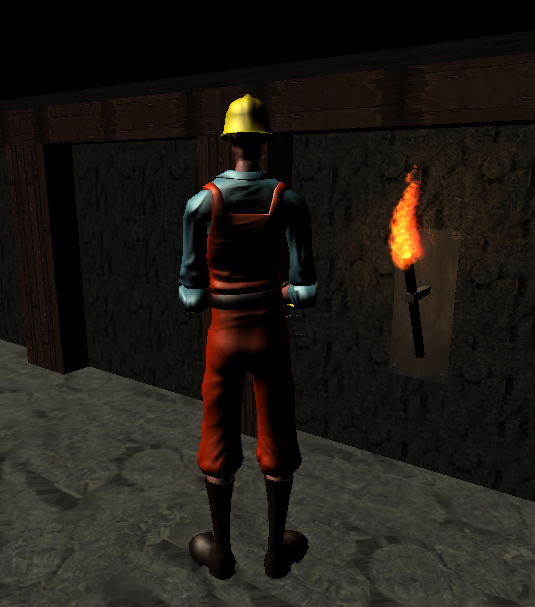
\includegraphics[width=9cm]{torche-ant.png}
	\end{figure}
	Le mineur dans le niveau d'Antoine
\end{center}



\newpage

\section{Cédric}
\paragraph{} \hspace{0pt} \\
Dès le commencement du projet, j’ai beaucoup travaillé pour trouver des idées pour le groupe.
J’ai appris rapidement à utiliser \LaTeX afin de rédiger le cahier des charges.
Dès le début du projet, je me suis appliqué à la réalisation du site web en PHP. 
Etant donné le fait que les offres d’hébergements ne nous convenaient pas, 
nous avons décidé de l’héberger nous-même ! Ainsi j’héberge le site internet sur un Raspberry PI 3. 
Je n’ai pas rencontré de problèmes mis à part qu’il a fallu trouver une solution pour faire tenir le câble Ethernet …

\paragraph{} \hspace{0pt} \\
Dès la fin du cahier des charges, j’ai créé le projet sous Unity et ai commencé à travailler.
J’ai tous d’abord commencé à organiser notre projet en créant des dossiers pour ranger nos scripts, 
nos modèles 3D, nos textures, nos scènes …
J’ai ensuite créé une porte avec son animation. J’ai eu un peu de mal à trouver comment fonctionnait 
le menu Animation d’Unity mais je me suis vite habitué et j’ai pu montrer comment créer une animation 
aux autres membres du groupe. J’ai ensuite créé un script pour ouvrir et fermer la porte : 
il suffisait de jouer l’animation pour permettre ces opérations.
Grâce à un collider sphérique attaché à la porte avec IsTrigger coché j’ai pu détecter 
si un joueur était dans ce collider (OnTriggerStay()) et donc si il pressait la touche E j’activait la dite porte.
Ensuite je me suis appliqué à la création du mineur puisque Edgar ne peut faire fonctionner Unity 
et que Clément avait un problème d’écran d’ordinateur. Le plus dur a été de trouver notre mineur !
La création du script pour le contrôle des mouvements était relativement simple puisque des fonctions 
comme Input.GetKey() permettent de savoir si la touche passée en paramètre est pressée !
Le script et le mineur créé, j’ai créé 2 joueurs :
{\begin{itemize}
	\item Le premier avec une vue à la troisième personne qui servira pour les cinématiques et quelques niveaux
	\item Un autre en vue à la première personne pour les niveaux  
\end{itemize}}

\paragraph{} \hspace{0pt} \\
J’ai ensuite commencé à m’intéresser au Network et j’ai installé Photon Unity Networking, 
J’ai ensuite tenté de créer le script du Network Manger. Après quelques heures de doute, 
nous avons pu jouer à plusieurs ! Bien que les animations ne soient pas synchronisées et que le rendu visuel des autres joueurs est un peu décalé et saccadé, cela fonctionne et nous réglerons ces problèmes plus tard.
Etant chef de projet, j’ai dû attribuer des tâches à chacun. 
Les troupes ont eu un peu de retard à l’allumage mais ils y sont mis vraiment début mai 
même si certains cherchaient toujours une issue pour éviter les tâches que je leur donnais.
Mais finalement, j’ai réussi à faire en sorte que nous soyons dans les temps !
J’ai aussi beaucoup aidé mes collègues à utiliser Unity ou à comprendre comment fonctionne les scripts C\# dans Unity.
\\
Cette première partie du projet m’as permis de découvrir le rôle de chef de projet.


\begin{center}
	\begin{figure}[!hp]
	   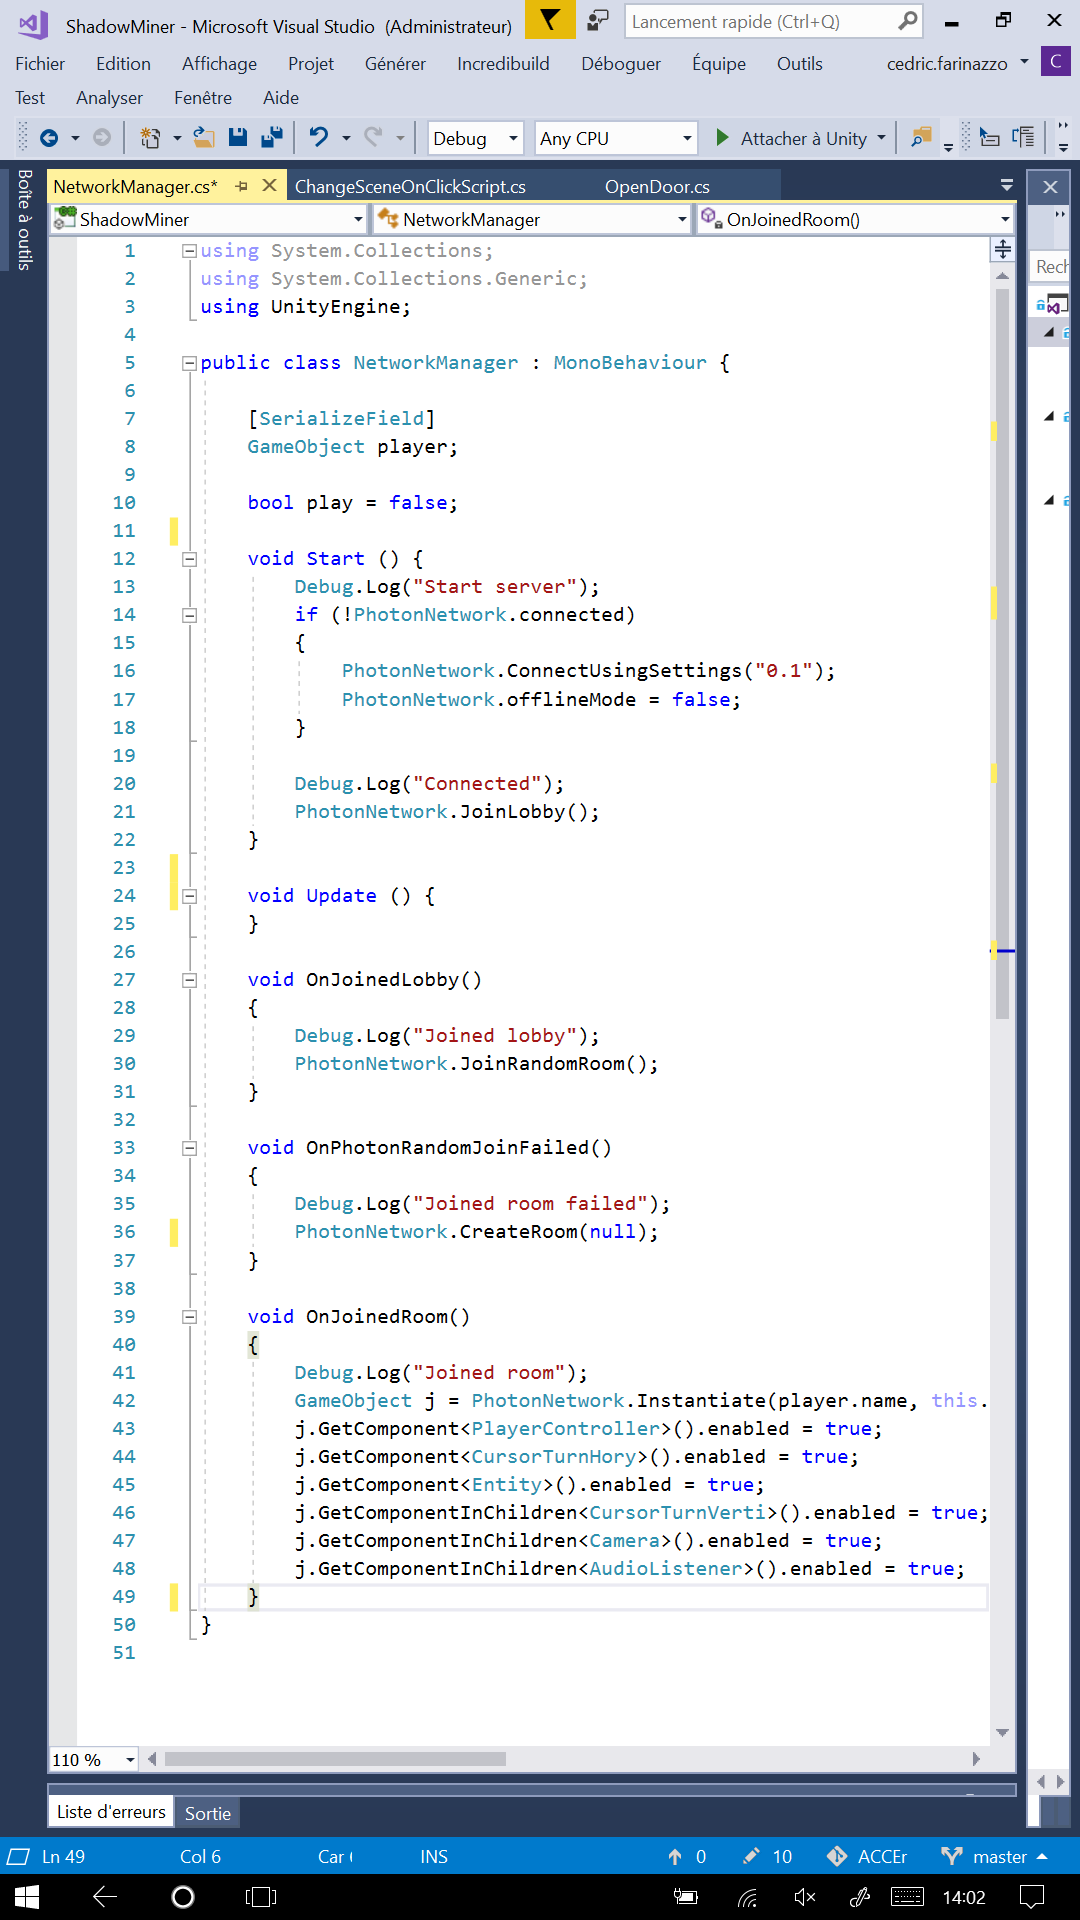
\includegraphics[width=10cm]{networkcs-game.png}
	\end{figure}
	Le script permmetant de se connecter au serveur multijoueur.
\end{center}


\newpage

\section{Clément}
\paragraph{} \hspace{0pt} \\
\begin{wrapfigure}[13]{r}{5cm}
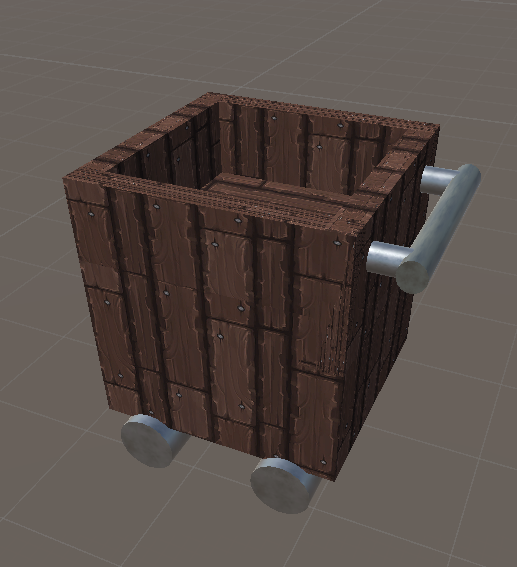
\includegraphics[width=5cm]{chariot-game.png}
\end{wrapfigure}
\begin{wrapfigure}[11]{r}{5cm}
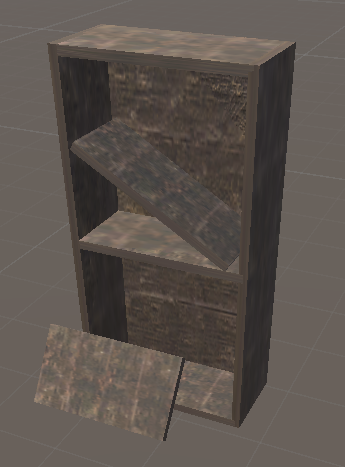
\includegraphics[width=5cm]{etagerecasse-game.png}
\end{wrapfigure}
Avant de commencer le projet, j'ai regardé des tutos Unity sur youtube et j'ai manipulé le logiciel en créant 
des préfabs de bases, puis des préfabs un peu plus complexes tels qu'un chariot, une étagère ou encore des 
planches en m'inspirant d'images du jeu Outlast 2. Puis j'ai commencé à mettre des textures à mes préfabs et,
à l'aide de Cédric, fait quelques animations comme celles du piège avec les pics qui sortent et rentrent d'un
préfab qui représente un sol. Il faut d'abord faire le préfab puis j'ai fait un script pour que le piège 
s'anime si un Player rentre dans le piège grâce à un collider et en cochant "Is Trigger" pour utiliser les
fonctions "OnTriggerEnter()" et "OnTriggerExit()" si le joueur sort du piège . \\


\begin{wrapfigure}[11]{r}{6cm}
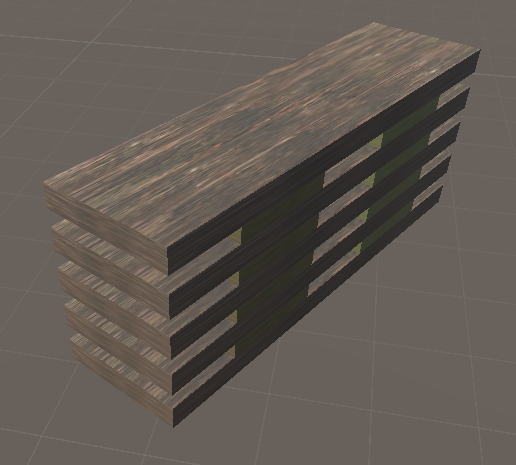
\includegraphics[width=6cm]{planche-game.png}
\end{wrapfigure}
Etant amateur de jeux, il est très fréquent que le joueur passe sous la map, notamment sur les jeux Unity 
(Hunt for Props par exemple), j'ai donc fait un système de respawn qui déplace le joueur à la position Y + 2
de la map du niveau.


\newpage

\begin{wrapfigure}[17]{r}{8cm}
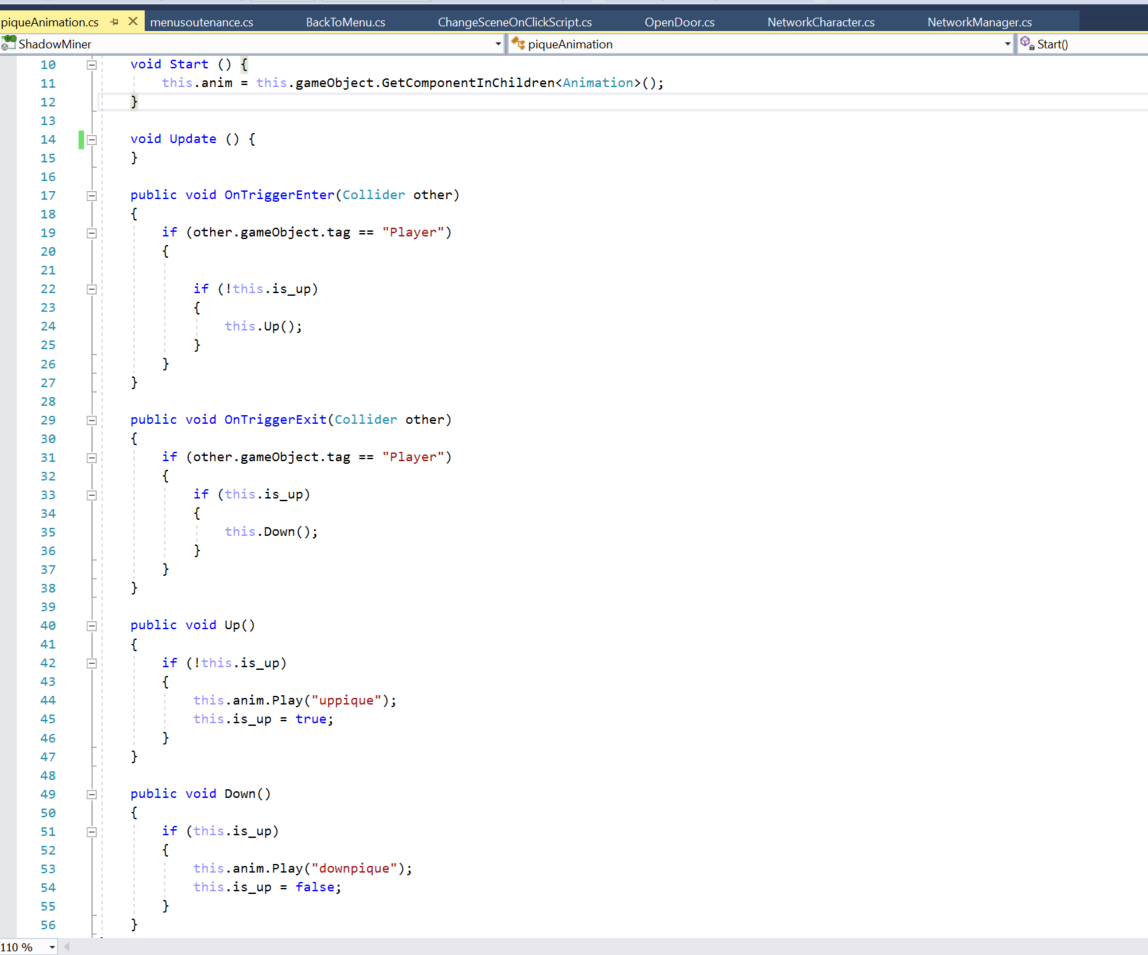
\includegraphics[width=8cm]{piquescript-game.png}
\end{wrapfigure}
Maintenant qu'on avait pas mal de préfabs, je pouvais commencé la confection du premier niveau. J'ai fait un plan du 
premier niveau (que j'ai toutefois modifié pour des raisons de design et de facilité pour un premier niveau).
En installant ProBuilder, Progrids et Polybrush, j'ai pu confectionné un terrain et faire le premier niveau. J'ai
créé des salles sans réels buts pour le moment et une boule se trouve à la fin du niveau pour accéder au menu (créée
par Antoine). Nous avons avec Cédric implémenter une musique pour rendre un peu plus dynamique les premiers niveaux 
(musique non définitives).

\paragraph{} \hspace{0pt} \\
  Pour la prochaine soutenance, je prevois de confectionner encore plus de préfabs (et ainsi enrichir le visuel 
des niveaux), créer de nouveaux pîèges et donc de nouvelles animations pour ces futurs pièges (hache qui sort du plafond, 
couteaux/flèches qui sortent du mûr ou encore le fameux rocher qui nous suit dans un long couloir). Un premier modèle d'une
map multijoueur et de nouveaux niveaux seront créés et les deux premiers seront améliorés.

\paragraph{} \hspace{0pt} \\
  Notre groupe est bien soudé, chacun a trouvé sa place. On a modifié les responsables et les suppléants dans la 
répartition des tâches (je veux créer pleins de préfabs!) car nous nous sommes rendus compte que certains voulaient faire le 
travail des uns et d'autres le travail des autres. Il a fallut attendre la semaine avant les Mid-terms (début mars) pour que 
je commence vraiment à me mettre dans le projet. Toutefois, à la découverte de Probuilder, ma vision du projet se métamorphosa
soudainement: je m'amusais avec les différentes formes. Toutefois, je me laisse facilement distraire par mes camarades de
projet pour leur donner mon avis (pas si distrait finalement car c'est un projet de groupe). J'ai pas mal travaillé avec Cédric
pour les animations des objets, les scripts et le multijoueur. Avec Antoine, on s'est échangé des idées et répartis la 
confection des différents préfabs et des deux premiers niveaux (qui sont alors complètements différents, mais qui donnent alors
une variété dans le visuel et le disign des niveaux).

\begin{center}
	\begin{figure}[!hp]
	   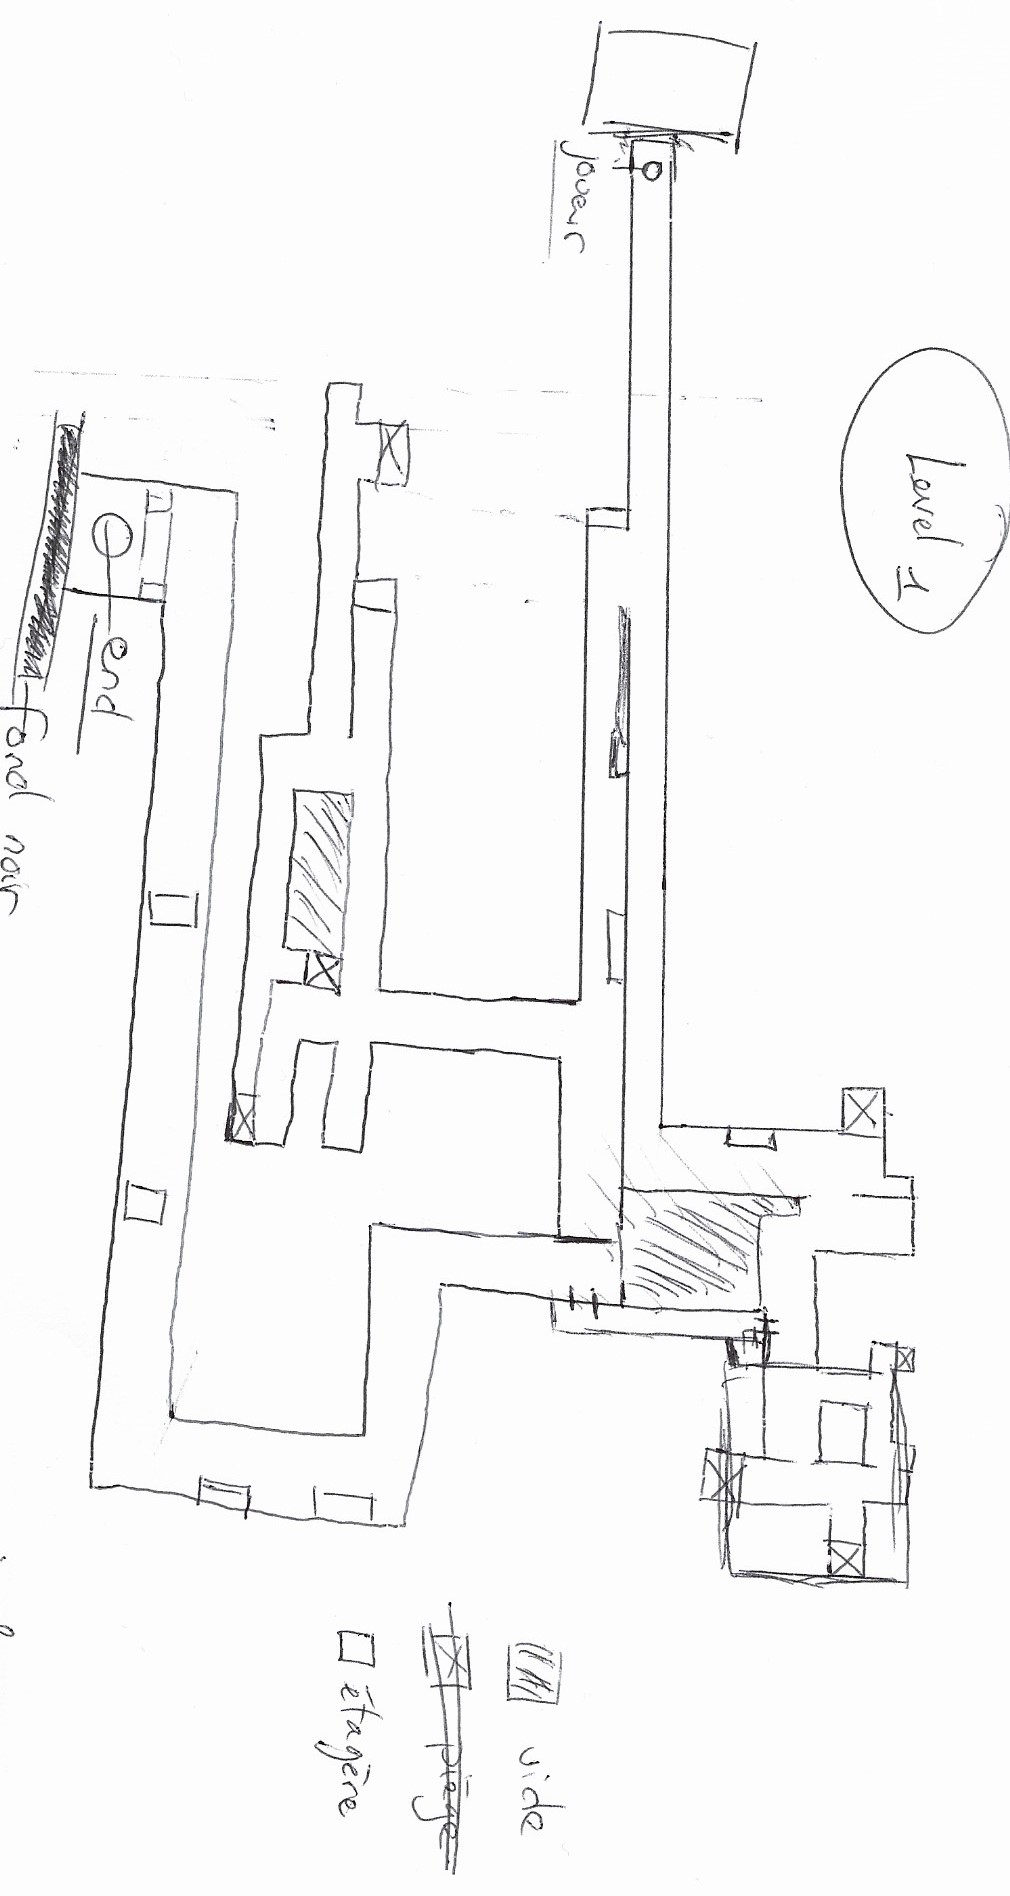
\includegraphics[width=10cm]{niveau-game.jpg}
	\end{figure}
	Maquette du niveau 1 réalisé par Clément
\end{center}


\section{Edgar}
\paragraph{} \hspace{0pt} \\
Edgar a eu beaucoup de mal pour travailler lors de la période avant la première soutenance.
En effet, son ordinateur est plutôt vieux et du coup Unity ne marche pas dessus. 
Cependant il ne s'est pas découragé et à quand même essayé d'aider son groupe pour certaines choses. 
Il a aidé faire le LaTeX et à tenter la création du Shadow Miner en essayant de créer celui en 3D grâce à Blender, 
malheureusement c'était un travail qui n'a servi à rien pour l'avancement du projet.
Il a créé les éboulis sur Unity, ces derniers jours quand il avait accès à ce logiciel.

\paragraph{} \hspace{0pt} \\
La première partie du projet lui a appris à mieux utiliser le language \LaTeX
malgré encore beaucoup d'erreurs. Il a surtout appris comment bien utiliser Blender pour faire de la modélisation 3D ce qu'il affectionne particulièrement. 
Edgar est extrêmement motivé pour ce projet car il fait quelque chose de concret et ça lui plaît énormément et il fait ce qu'il aime

\paragraph{} \hspace{0pt} \\
Sur le mois qui suit, Edgar est extrêmement motivé à faire le son du jeu ainsi que enregistrer des sons dans la nature comme des bruits de pas ou 
des grognements ou plein d'autres choses qui peuvent aider le jeu à être plus réel il aidera aussi à faire le script en c\# pour le joueur 
ainsi que de débuter la création du système de map aleéatoire pour le multijoueur.

\newpage
\part{Organisation du projet}
\paragraph{} \hspace{0pt} \\ 
Nous avons jugé utile de mettre à jour ce tableau de répartition des tâches
\\ \\
{\normalsize
	\begin{tabular}{|p{6cm}|p{1.2cm}|p{1.2cm}|p{1.2cm}|p{1.2cm}|}
		\hline
		Tâches & \multicolumn{4}{|c|}{Personnes} \\ 
		\cline{2-5}
			& Antoine & Cédric & Clément & Edgar \\
		\hline
		Création des préfabs de map pour les niveaux (murs, sol, porte, ..) & Supp\footnotemark[2] & X & Resp\footnotemark[1] & X \\
		\hline
		Modélisation 3D pour de meilleurs graphismes (si possible) & Supp\footnotemark[2] & X & X & Resp\footnotemark[1] \\
		\hline
		Script c\# animation & X & Resp\footnotemark[1] & Supp\footnotemark[2] & X \\
		\hline
		Création des préfabs des joueurs & Supp\footnotemark[2] & Resp\footnotemark[1] & X &  \\
		\hline
		Script c\# joueur & X & Resp\footnotemark[1] & X & Supp\footnotemark[2] \\
		\hline
		Création de multiples niveaux (entre 20 et 40) & Resp\footnotemark[1] & X & Supp\footnotemark[2] & X \\
		\hline
		Création du Shadow Miner et Script c\# pour l'IA du Shadow Miner & X & Resp\footnotemark[1] & X & Supp\footnotemark[2] \\
		\hline
		Cinématique du jeu & X & X & Resp\footnotemark[1] & Supp\footnotemark[2] \\
		\hline
		Son du jeu & X & X & Supp\footnotemark[2] & Resp\footnotemark[1] \\
		\hline
		Menu du jeu & Resp\footnotemark[1] & X & Supp\footnotemark[2] & \\
		\hline
		Création du site internet et Hébergement en ligne & X & Resp\footnotemark[1] & X & Supp\footnotemark[2] \\
		\hline
		Création du serveur multijoueurs & Supp\footnotemark[2] & Resp\footnotemark[1] & X & X \\
		\hline
		Création des joueurs pour multijoueurs & Supp\footnotemark[2] & Resp\footnotemark[1] & X & X \\
		\hline
		Création du système de map aléatoire pour le multijoueurs & Supp\footnotemark[2] & X & X & Resp\footnotemark[1] \\
		\hline
		Compte rendu en \LaTeX & X & Resp\footnotemark[1] & X & Supp\footnotemark[2]  \\
		\hline
		Compilation du jeu et enregistrement sur CD & X & X & Resp\footnotemark[1] & Supp\footnotemark[2] \\
		\hline
		Création trailer , plaquette et manuel d'installation et d'utilisation du jeu & X & X & Supp\footnotemark[2] & Resp\footnotemark[1] \\
		\hline
	\end{tabular}
	\label{repartition}		
	\footnotetext[1]{Responsable}
	\footnotetext[2]{Suppléant}
}

\newpage
\part{Autre image du jeu}
\begin{center}
	\begin{figure}[!hp]
	   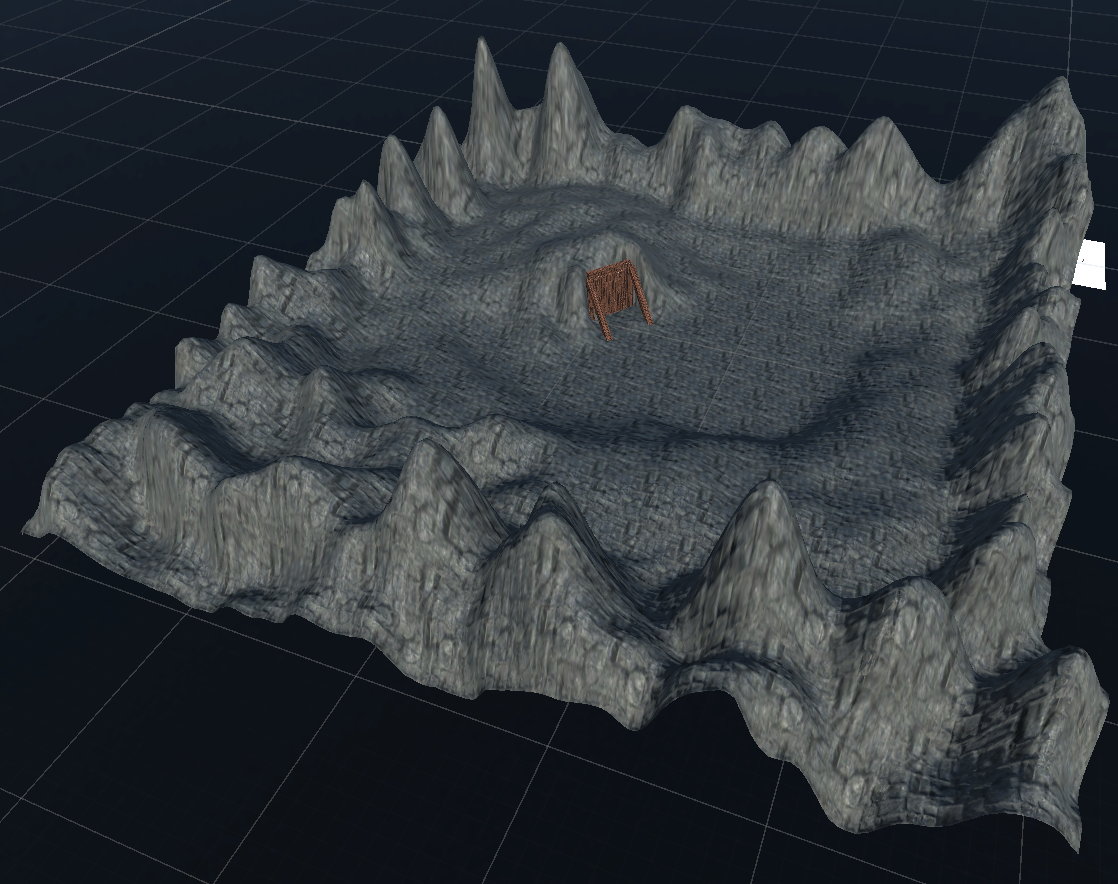
\includegraphics[width=10cm]{mine-game.png}
	\end{figure}
	L'extérieur de la mine réalisé par Cédric
\end{center}

\newpage

\part{Conclusion}
Nous avons bien avancé et nous avons remplis nos objectifs.
Les personnage sont en place ainsi que 2 niveaux et le multijoueur.
\\ \\
Nous comptons donc continue dans cette voie en continuant le multijour, la création de préfabs, la modélisation 3D d'objets, 
la création du profile du joueur et de la sauvegarde de sa progression.
\\ \\
Ce projet nous tient tous à coeur et nous voulons nous dépasser afin d'obtenir ce que nous voulons ! 

\end{document}